% Chapter 2

\chapter{On-Stack Replacement} % Main chapter title

\label{Chapter2} % For referencing the chapter elsewhere, use \ref{Chapter2} 

%----------------------------------------------------------------------------------------

% Define some commands to keep the formatting separated from the content 
\newcommand{\keyword}[1]{\textbf{#1}}
\newcommand{\tabhead}[1]{\textbf{#1}}
\newcommand{\code}[1]{\texttt{#1}}
\newcommand{\file}[1]{\texttt{\bfseries#1}}
\newcommand{\option}[1]{\texttt{\itshape#1}}

%----------------------------------------------------------------------------------------
This chapter introduces on-stack replacement.
The first section provides an overview of on-stack replacement principles.
The second section presents on-stack replacement mechanisms, and defines OSR related vocabulary.
The third section focuses on the use of on-stack replacement for runtime deoptimization.
Finally, the fourth section summarizes constraints on OSR implementations.\\

\section{Overview}
\subsection{Definition}

On-stack replacement (OSR) refers to a runtime compiler transformation technique that allows to replace a program that is executing by another program.
OSR implementations allow to interrupt running code during the execution of a function, transform it, e.g., reoptimize it, and resume the execution in the new function at the correct instruction and state.
The action of transferring the execution using the OSR mechanism is called a \textit{transition}.\\

On-Stack replacement can be viewed, at a high level, as a mechanism that allows to transform the currently executing function into another version of itself.
This transformation mechanism has been used to allow transitions between different levels of code optimizations.
We can therefore reduce it to two main purposes: (1) transforming an executing function into a more optimized version of itself, and (2) undoing transformations that were previously performed.
While similar, these two types of transformations have very different goals.\\

In several virtual machines~\cite{paleczny2001java, lameed2013modular, holzle1992debugging, fink2003design, soman2006efficient, duboscq2014speculation, OSRKit, WebKitFTL}, some of which will be presented in Chapter \ref{Chapter3}, on-stack replacement has been used to improve the performance of long running functions.
When the virtual machine (VM) identifies a piece of code as being "hot", i.e., it hogs the execution, the VM suspends the function's execution, recompiles it to a higher level of optimization, and transfers the execution to the newly generated version of the function.
This differs from a simple Just-In-Time (JIT) compiler, since the recompilation and transfer of execution both take place during the execution of the function, rather than just before it.
However, both techniques rely on the same assumption, namely, that runtime profiling data enables to uncover new optimization opportunities.\\

On-Stack replacement allows a compiler to perform speculative transformations.
Some optimizations rely on assumptions that are not bound to hold during the entire execution of a program.
A simple example is function inlining in an environment where functions can be redefined at runtime.
A regular, and correct, compiler would not allow to inline a function that might be modified during the execution.
The OSR mechanism, however, enables to perform such an optimization.
Whenever the assumption fails, i.e., the function is redefined, the OSR mechanism will enable to transfer the execution to a corresponding piece of code where the inlining has not been performed.
In this case, OSR is used to allow potentially erroneous transformations while preserving correctness.\\

In summary, on-stack replacement is a powerful technique that can be used to either improve performance, or enable speculative transformations of the code while preserving correctness.
The next section presents the advantages that OSR uncovers in both cases.

\subsection{On-Stack Replacement Benefits}\label{WhyOSRInteresting}
%The optimization case
     %wait until enough profiling information is gathered to make some new assumptions and improve code quality
    %Some enable to have several specialised versions of the code live at the same time.
    %Chaining OSR means that we can keep optimising the code -> depends on profiler
%The deoptimization case
    %This is the real deal. optimization is not valid without this counter part. 
    %Enables even more agressive code specialisation. Being able to undo means that we can have virtually any assumption and just revert back to a safe version if it fails. 
    %The real difference: optimization is for performance, deoptimazation is for correctness.
    
%This section highlights the benefits of using on-stack replacement, with respect to both otpimization and deoptimization.\\

On-Stack replacement increases the power of dynamic compilation.
A function can be recompiled while it is executing.
This enables more aggressive adaptative compilation than just-in-time (JIT) compilation.
In fact, the OSR mechanism, in theory, allows to perform a recompilation at any instruction boundary. 
As an adaptative compilation mechanism, it enables to delay the compilation of a code artefact and therefore enables to gather more information about the current execution profile.
These information can then be used to produce higher quality compiled code, with better execution performances.\\

For dynamic languages, code specialization is an efficient technique to improve performances~\cite{gal2009trace}.
Code specialization consists in tuning the code to better fit a particular use case and set of types, hence yielding better performances.
Specialization can be viewed as a mechanism relying on the versioning of some piece of code.
One of the main challenges is to identify which version better fits the current execution need.
This requires to gather enough profiling information, some of which might not be available until some portion of the code is executed multiple times.
On-stack replacement enables to speculatively specialize code, while preserving the program's correctness.\\

OSR, coupled with an efficient compiler to generate and keep track of specialized functions, enables to uncover new opportunities to fine tune a portion of code.
While techniques like JIT compilation can generate specialized code at a function level, i.e., before the function's execution, OSR enables to make such tuning while a function is running.
For example, in the case of a long running loop inside a function, JIT techniques would need to wait until the function is called anew to improve its run time performance by recompiling it. 
OSR, on the other hand, gives the compiler the means to make such improvements earlier, hence yielding a better overall performance of program's execution.\\

OSR mechanisms enable the compiler to recompile and optimize at almost any time during the execution of a program.
A clever compiler can perform iterative recompilation of the code in order to improve the quality of the generated compiled artefact.
OSR enables these iteration steps to be closer to each other and potentially converge to a better solution faster than other dynamic compilation techniques.\\

On-Stack replacement's most interesting feature is deoptimization. 
While optimization enables to increase performance, deoptimization's goal is to preserve the program's correctness in the presence of aggressive speculative optimizations. 
Virtually any assumption can be used to generate compiled code and, if the assumption fails, 
OSR enables to revert back to a safe version during the execution.\\

\section{Terminology \& Mechanisms}

\subsection{Transition Points}\label{section:osrpoints}
%TODO do a definition case for that
%Several names for it 
%what it is: a point in the code from which we can suspend the exec and optimize the current version of the code
    %Implies that we need a "safe state”, i.e., we need to be able to find an equivalent point in the optimized version
    %portions of code that don’t have interrupts
    %Too many -> bad Too few -> bad
%Guarded vs Unguarded 
    %Guarding when there is an explicit condition that we can check locally
    %What if global/External event? 
        %Some have a map of such points and fix them whenever an external event happens (citing papers e.g., jikes)
%OSR exits 
    %What to do when the condition fails? 
        %optimization dependent 
        %for external requires to correct every callee return landing spots. 
        %Requires corresponding entry in the unoptimized version
%Examples from existing implementations 
    %McOSR inserter and instrument passes (need a code transformer + OSR Label)
    %Jikes
On-stack replacement is enabled at specific instruction boundaries in the user's code.
Depending on the implementation, these points can be sparse, restricted to special points in the program control flow, or associated with special framework dependent data.
In the literature, such boundaries were given various names, e.g., \textit{interrupt points}~\cite{holzle1992debugging}, \textit{OSR points}~\cite{fink2003design, holzle1992debugging, WebKitURL, lameed2013modular}, \textit{OSR entries}, and \textit{OSR exits}~\cite{WebKitURL, lameed2013modular}.
This section presents the terminology for such points that will be used in the reminder of this report.

\begin{definition}\label{OSRPointDefinition}
An OSR point is a portion of code that belongs to the OSR instrumentation.
It is located at an instruction boundary at which the program can be suspended.
OSR points can correspond to several instructions and enable to perform the transition from one version of the code to another.
\end{definition}

%TODO continue this part by explaining why we need it to be safe
An OSR point has to be located at a point of the code where the state is \textit{safe}, i.e., instruction boundaries where the state is guaranteed to be consistent.
For example, as explained in section \ref{SELF}, the SELF debugger~\cite{holzle1992debugging} considers points at method prologues and at the end of loop bodies.
An OSR point must be such that the state of the computation can be extracted and transferred to another version of the code from which the execution can resume.
As a result, different implementations yield different restrictions on the location of OSR points.\\

\subsubsection{Guarded \& Unguarded}

OSR points can be divided into two categories: \textit{guarded} and \textit{unguarded}.
\begin{definition}
A guarded OSR point's execution depends on an explicit boolean test, called the OSR condition.
In other words, the framework has enough information locally to test whether or not an OSR transition should be taken.
\end{definition}
\begin{definition}
An unguarded OSR point does not require to locally check a boolean condition before being executed. 
\end{definition}
The distinction between guarded and unguarded points is present in the literature (e.g., Jikes RVM~\cite{fink2003design, soman2006efficient} and WebKit~\cite{WebKitURL}).
Both solutions present different advantages and fit different use cases.\\

While simple to model at a high-level, a guarded OSR point presents the disadvantage of increasing the code's length. 
A boolean condition needs to be tested every time the execution comes across an OSR point.
As a result, the repeated evaluation of conditions might undermine the performance improvements obtain via on-stack replacement, especially in the case of long running loops optimization.\\

Unguarded OSR points enable to avoid this overhead by letting the framework modify the running function on external/environmental events.
WebKit~\cite{WebKitURL}, for example, overwrites portion of the compiled code, at runtime, in order to introduce an unconditional transition.
This can be viewed as a lazy triggering of on-stack replacement, i.e., the instrumentation to enable the transition can be added just before being executed.\\

\subsubsection{Entries \& Exits}

There is a further distinction between OSR points that are responsible for optimizing the code, and the ones that are used to deoptimize.
We adopt the same terminology as in WebKit~\cite{WebKitURL} and McOSR~\cite{lameed2013modular}.

\begin{definition}\label{OSREntryDefinition}
An OSR point that enables to replace the current version of the code with one in which we expect to have better performance is called an \textbf{entry}.
OSR entries are used in the optimization process.
\end{definition}

\begin{definition}
An OSR point that enables to exit the current version of the code when it is invalidated is called an \textbf{exit}.
OSR exits are responsible for preserving the correctness of the program.
They are used in the deoptimization process.
\end{definition}

At the implementation level, OSR entries and exits are very similar, if not identical. 
They both are OSR points and will trigger a transition.
Conceptually, however, an exit is part of the mechanism that enables to protect the correctness of the program.
Mistakingly not taking an entry is a missed opportunity for better performances.
Missing a required exit leads to a possibly incorrect behavior of the program.\\

\subsection{The Transition}
On-stack replacement's core functionality is to allow a transition, at runtime, from the middle of a running function to a corresponding instruction in the middle of another version of this function.
This transition mechanism is therefore the cornerstone of any OSR implementation.
This section strives to unify all the existing implementations under a single, general, high-level list of requirements to perform an OSR transition.\\

In the reminder of this section, we use the terminology introduced by definitions \ref{from}, \ref{base}, and \ref{continuation}, and taken from the OSR Kit~\cite{OSRKit} project.
These definitions hold, regardless of the type of OSR transition, i.e., OSR exit or OSR entry, being performed.\\

\begin{definition}\label{base}
A base function is a non-instrumented function. 
It serves as a base input for compiler transformations and on-stack replacement instrumentations.
\end{definition}

\begin{definition}\label{from}
A function from which we perform a transition is called a \textbf{from function} or \textbf{source version}.
\end{definition}

\begin{definition}\label{continuation}
A function in which we resume the execution after a transition is called a \textbf{continuation function} or \textbf{destination version}.
\end{definition}

\subsubsection{High-Level requirements and challenges for transitions}\label{HLREQ}
%OSR transition is a mapping
    % mapping = reconstruct the state 
        %what it means to reconstruct the state: live values
        % what if opt introduces new values ?
    %mapping = find the correct instruction to which
%An OSR transition is transparent
    %Should be triggered without the user intervention
    %Requires to deviate from regular execution path. 
%OSR transition can be biderectional

An OSR transition relies on a mapping between two program points and their respective states.
Such a mapping is possible only if all the information available at the OSR point in the from function is sufficient to reconstruct the state expected at the landing site in the continuation function.\\

Reconstructing the state at the landing site means that all the expected live variables must be assigned  correct values to safely resume the execution in the continuation function.
Propagating live values is, itself, a challenge, and requires to keep a mapping between the live values in the from function and the live values in the continuation function.
Compiler optimizations might eliminate variables, fuse them, create new ones, and hence prevent a one-to-one mapping between the two sets of live values. 
As a result, the OSR transition implementation must provide a function \textit{f} that takes as input the set of live variables and their assigned values $S_s$ from the source version \textit{s} and generates a new set of live variables mapped to their values $S_d$ for the destination version \textit{d}.

\[f: S \rightarrow S\]
\[f(S_s) = S_d\]

An OSR transition is transparent to the user, i.e., it should not be observed by the user running the program.
The OSR transition can be viewed as a mechanism that deviates the program from its current execution path in order to either improve the runtime performance or preserve correctness.
It is part of the compilation/execution framework and, aside from a performance variation, should not impact the execution of the program, e.g., a correct program should not crash because of an OSR transition.\\

An OSR transition can be either \textit{unidirectional} or \textit{bidirectional}.
In the case of a bidirectional mapping between the source and the destination version, the framework must also provide a function \textit{f'} that is the inverse of \textit{f}.  
\[f': S \rightarrow S\]
\[f'(S_d) = S_s\]
If the source is a less optimized version of the destination, $f'$ is used during the deoptimization case.
The deoptimization case presents a greater challenge than the optimization one.
Consider the unoptimized code in Figure \ref{unoptimizedcase}, and its optimized version in Figure \ref{optimizedcase}.

\begin{figure}[h]
\centering
\begin{subfigure}{.49\textwidth}
  \centering
  \begin{lstlisting}
a <- 5
b <- 6
c <- a+b
    \end{lstlisting}
  \caption{Unoptimized case}
  \label{unoptimizedcase}
\end{subfigure}%
\begin{subfigure}{.49\textwidth}
  \centering
  \begin{lstlisting}
  
  
c <- 11
    \end{lstlisting}
  \caption{Optimized case}
  \label{optimizedcase}
\end{subfigure}
\caption{Variable elimination example.}
\label{variableEliminationExample}
\end{figure}


The function \textit{f'} must provide a way to re-generate \codekey{a} and \codekey{b} from \codekey{c}. 
To this end, it must remember the steps that led to the optimized version of the code, and must be able to reverse them.
This implies a lot of metadata attached to each version of the optimized code generated by the compiler and might quickly increase the space complexity of the OSR support.
The VARMAP structure in the Jikes RVM~\cite{soman2006efficient} and the scope descriptors in SELF debugger~\cite{holzle1992debugging} are examples of such metadata attached to the code that enable to recover the values of \codekey{a} and \codekey{b} from \codekey{c}.\\
 
\subsubsection{The low-level transition}
%low-level transition description.
%hit the point
    %save the register content.
    %modify the stack to have expected values, calls made by the other function
    %put register content
    %modify program counter and resume execution
%Hard if do not have complete control over the execution platform, and still need to be able to understand machine level meaning of the code etc.
At a machine code level, an ideal OSR transition can be summarised into 5 steps: 
\begin{enumerate}
    \item Save the content of the registers.
    \item Save the local live values, i.e., the on-stack values in the current stack frame.
    \item Modify the current stack frame to introduce the expected local values, add expected stack frames or remove the stack frames that are not needed.
    \item put the correct content inside the registers.
    \item modify the program counter and resume the execution.
\end{enumerate}\\

There exists several examples of OSR implementations that manipulate the program state at machine code level to allow the continuation function to execute in the current stack frame~\cite{chambers1991making, holzle1992debugging, suganuma2006region}.
In order to perform such a modification of the runtime stack and registers, the framework must have extensive control over the machine executing the program.
This requirement is easier to satisfy if the execution is performed inside a virtual machine that enables to access and modify the execution stack and the registers.
Section \ref{OSR&VM} expands on the relation between OSR implementations and virtual machines.
Furthermore, as explained in \ref{HLREQ}, reconstructing a state from a set of live values is challenging. 
Performing this operation at such a low level is hard.
The compiled version of the code loses the high-level semantics specific to the language, translates some high-level operations into several sequential instructions and performs some low level ressource management (e.g., register allocation) that requires the OSR mechanism to perfectly understand how the compiled code is generated in order to enable the transition at machine code level.\\

While tempting for its fine-grained control over the transition, the implementation of the OSR mechanism at a low level seems to unveil great challenges.
An alternative solution is to encapsulate the entire process at a higher level, closer to the original program's semantics.\\

\subsubsection{The transition as a function call}
%A function call at a high level
    %In fact, a function call is the basic way of jumping to another portion of code
    %Propagate the state
        %load it 
        %pass it as arguments to the call.
    %Single entry point to the continuation function means for each spot we need a function
    %Multiple entry points
An OSR transition can be modelled as a function call.
As explained previously, a transition needs to propagate values and jump to a continuation point outside of the current execution path.
A function call allows to modify the program counter and jump to another portion of code.
The OSR transition can therefore be viewed as a tail function call from the source version to the destination version containing the newly generated code.\\

There exist two different ways to propagate the current execution state:
\begin{enumerate}
    \item Dumping the state in a shared memory location (e.g., as in the McOSR implementation~\cite{lameed2013modular} and WebKit~\cite{WebKitURL}), or
    \item Passing all the needed values as function call arguments to the continuation function(e.g., as in OSR Kit~\cite{OSRKit} and Jikes RVM OSR~\cite{fink2003design}).
\end{enumerate}

The first option implies that the from function must dump its state into a buffer before calling the continuation function.
The continuation function starts its execution by loading the values it needs from the buffer.
This solution has the drawback of increasing both the from function and the continuation function lengths, i.e., the propagation of the state has a greater impact on the program's execution time than a simple function call cost.
Figure \ref{fig:bufferExample} provides a simple example of an OSR mechanism, implemented as a function call, that relies on a buffer to propagate the state in the continuation function.
In the from function Figure \ref{fig:fromFuncBuff}, lines 10 to 13 enable to save the current state in a shared buffer.
In the continuation function, i.e., Figure \ref{fig:ContFuncBuff}, lines 4 to 7 load the state from the buffer.\\

\begin{figure}[h]
    \centering
    \begin{subfigure}{.49\textwidth}
        \includecode{Code/bufferFrom.c}
        \caption{From function.}
        \label{fig:fromFuncBuff}
    \end{subfigure}
    \centering
    \begin{subfigure}{.49\textwidth}
        \includecode{Code/bufferCont.c}
        \caption{Continuation function.}
        \label{fig:ContFuncBuff}   
    \end{subfigure}
    \caption{Using a buffer to pass live values in an OSR transition.}
    \label{fig:bufferExample}
\end{figure}

For the second option, most of the work needed to propagate the state is performed during the compilation.
Values are passed as arguments to the call to the continuation function.
If there is not a one-to-one mapping between the from variables and the continuation ones, some compensation code is executed, either before the call or at the beginning of the continuation function, in order to assign the correct values to the continuation local variables.
The cost of executing the compensation code is also present in the first option, i.e., both solutions have to perform the same set of transformations in order to generate the expected local values.
On the other hand, the second option does not require to access shared memory to store and load propagated values, and is therefore expected to have a smaller cost at execution.
Figure \ref{fig:CallExample} provides the same OSR transition as in Figure \ref{fig:bufferExample}, but passes live values as arguments to the continuation function.\\

\begin{figure}[h]
    \centering
    \begin{subfigure}{.49\textwidth}
        \includecode{Code/callFrom.c}
        \caption{From function.}
        \label{fig:fromFuncCall}
    \end{subfigure}
    \centering
    \begin{subfigure}{.49\textwidth}
        \includecode{Code/callCont.c}
        \caption{Continuation function.}
        \label{fig:ContFuncCall}   
    \end{subfigure}
    \caption{Live values as arguments in an OSR transition.}
    \label{fig:CallExample}
\end{figure}

%multiple entries
\begin{figure}[h!]
\centering
\begin{subfigure}{.8\textwidth}
\includecode{Code/MultipleEntry.c}
\end{subfigure}
\caption{Instrumented function with multiple entry points.}
\label{fig:multipleentry}
\end{figure}

The transition requires to enter the continuation function at a special instruction that corresponds to the OSR point in the from function.
In order to decrease the space complexity, one might want to enable multiple entry points per function.
Consider Figure \ref{fig:multipleentry}, where \codekey{fbase} provides three entry points: (1) the regular entry point \codekey{ENTRY}, (2) a continuation \codekey{CONT1} and (3) a second continuation \codekey{CONT2}.
The function \codekey{fbase} can therefore be used as a continuation function for any from function that has an OSR transition from a point that corresponds to either \codekey{CONT1} or \codekey{CONT2}, as well as for regular function calls.
In order to allow multiple entry points, the \codekey{fbase} is instrumented, i.e., a prologue block is executed at its beginning.
The prologue is responsible for identifying \codekey{fbase}'s caller. 
In Figure \ref{fig:multipleentry}, this is done by checking the value of a general flag, called \codekey{OSR\_LABEL}.
According to this value, it then jumps to the correct instruction inside the function, and, if an OSR transition is being performed, loads the state from the shared buffer, as described before.\\

The instrumentation for multiple entries per function has an impact on performance, as it requires an extra computation at the beginning of the function. 
On the other hand, the second technique that we described to propagate the state modifies the function's signature.
If the set of values to propagate is different at two points, we need different functions, and hence, should allow only a single entry point for each continuation function.
Therefore, we can expect the second solution to have, in general, a higher space complexity (i.e., many versions of the function live in memory at the same time) but a better performance during execution (i.e., smaller execution time).\\

\subsection{Versioning}
On-stack replacement requires, at some point, to have at least two versions of a function: the from function and the continuation function.
Furthermore, the continuation function can either be generated on the fly, i.e., the OSR transition includes a transformation step to generate the correct continuation function, or a previously compiled and cached version can be used.

\subsubsection{One version}
%Replace in place
%Good for space
%Jikes on the fly, interpreter kind of on the fly. 
Allowing only one live compiled version of the function enables to simplify the high-level model of the program's execution.
Some OSR implementations, such as the McOSR~\cite{lameed2013modular}, replace the from function with the continuation one in-place, i.e., the continuation function is compiled and registered at the from function's address.
This technique enables to propagate the optimized version through out the code without requiring any modification of the callers.
One can view it as an eager propagation of optimizations.
The overall performance of the execution should be improved by the global use of this optimized version.
On the other hand, this technique requires to ensure that any OSR entry taken is based on a condition that holds at any possible call site of the function.
It might therefore prevent function specialization in local sub-scopes.
Moreover, depending on the OSR implementation, it might require to trigger an OSR transition for frames in the middle of the execution stack.
\\


\subsubsection{Multiple Versions}
%Fine grain specialization
%Hard to keep track ? 
%For deoptimization it is a requirement since hard to reverse an opt transformation
    %Even harder if several opt performed NEED THAT OR NOT?
Fine-grained specialization of functions enables to improve performance locally.
In fact, allowing multiple versions of the same function to be live at the same time enables to optimize a function according to local conditions, regardless of other call sites states.
While attractive for the extra flexibility it provides, this solution presents several disadvantages.
First, it might increase space complexity.
In fact, allowing such specialization might lead to having one version per call site.
If not carefully handled, this can dramatically increase memory usage.
Second, this technique is a lazy propagation of optimizations.
Assume different calls to the same function.
In one call execution, call it $C_1$, an OSR condition allows to take a specific OSR entry.
Other calls, that will take the same OSR entry, do not benefit from the OSR condition tested by $C_1$, i.e., they will have to wait until they reach the same entry, and verify the same condition, before taking the transition.



\subsubsection{Caching vs. Generating on the fly}
%About caching and generating on the fly
%How much reusability really?

Depending on the reusability of a function's version, and its likelihood to be needed later in the execution, a time vs. space complexity trade-off appears.
Generating a continuation function on the fly is time consuming.
If the same OSR entry is taken multiple times, and leads to the same version of a function, caching this version might improve runtime performances.
On the other hand, if OSR entries are rarely taken, i.e., if OSR transitions are rare, generating the continuation function on the fly enables to save memory space. 
The cost of the compilation is amortised by the improvements allowed by the optimization and the live range of the function. 
In other words, generating on the fly is viable if the time performance gain of the optimized version over the entire execution is larger than the time required to generate the continuation function.
Furthermore, generating the continuation function on the fly enables to take into account the latest profiling data gathered about the program's execution and use it during the compilation.\\

%SHOULD I SAY SOMETHING ABOUT HOW PROGRAM SPECIFIC THAT IS? 

\section{On-Stack Replacement Deoptimization}
%TODO NOT SURE ABOUT GREATE CHALLENGE...
This section presents an overview of the deoptimization case with on-stack replacement.
OSR deoptimization presents several interesting design decisions and trade-offs.

\subsection{Deoptimization Benefits}\label{WhyDeopt}
%TODO for correctness
%Enable aggressive adaptive optimizations
%Relies on the quality of profiler and assumptions made
On-stack replacement main interest lies in dynamic deoptimization of code.
A compiler, equipped with an efficient implementation of OSR, is allowed to perform adaptive optimizations, based on some assumptions that might fail at some point during the execution.
Put in another way, OSR enables aggressive speculative optimizations of code by providing a mechanism that preserves correctness.\\

On-stack replacement enables to perform optimizations which are common in static languages compilers, but unsound in dynamic languages.
Function call inlining, for example, is a common optimization performed in static programming languages compilers. 
It enables to eliminate the overhead of a function call and return, and enlarges the scope considered for further optimizations.
While very common in static languages, inlining proves to be more difficult to implement in compilers for dynamic languages, if functions can be redefined at runtime.
OSR allows to perform speculative inlining of function calls. 
The assumption taken by the compiler is that the function call corresponds to a specific function body. 
A guarded OSR point checks that the inlined function was not redefined before executing the inlined body.
If the assumption fails, i.e., the function was redefined, the OSR mechanism allows to exit to a version of the code where the call was not inlined.\\

The OSR mechanism is a tool, which efficiency depends on the quality of the assumptions made.
This is even more visible in the deoptimization case.
The optimization case remains useful for regular optimizations, i.e., an OSR entry can be allowed by some profiling data gathered during the execution, and based on some fact that will hold for the rest of the execution.
On the other hand, an agressive assumption-based optimization exposes a trade-off between the performance improvement that it allows on one side, and the cost it has in the case of an assumption failure on the other.
As a result, the OSR deoptimization process allows a greater flexibility but should be coupled with an efficient profiler in order to identify cases where and when the program's execution might benefit from aggressive speculative optimizations.\\

\subsection{The Exit Target}
%Interesting because flexibility in where to exit.
%Depending on the trade off between time we can spend generating the exit, control over the environment etc.
%This section describes different options.
The OSR deoptimization case is interesting in the latitude it leaves with regard to where the optimized code should exit.
In the OSR entry case, the continuation function is a more optimized version of the code.
In the OSR exit case, there is still a choice to make: should the continuation function be a fully unoptimized version of the code? Or should we strive to obtain the most optimized and correct version of the code?
This section describes several targets for OSR exits, and tries to present the advantages, disadvantages, and requirements for each option.\\

\begin{figure}[h]
\centering
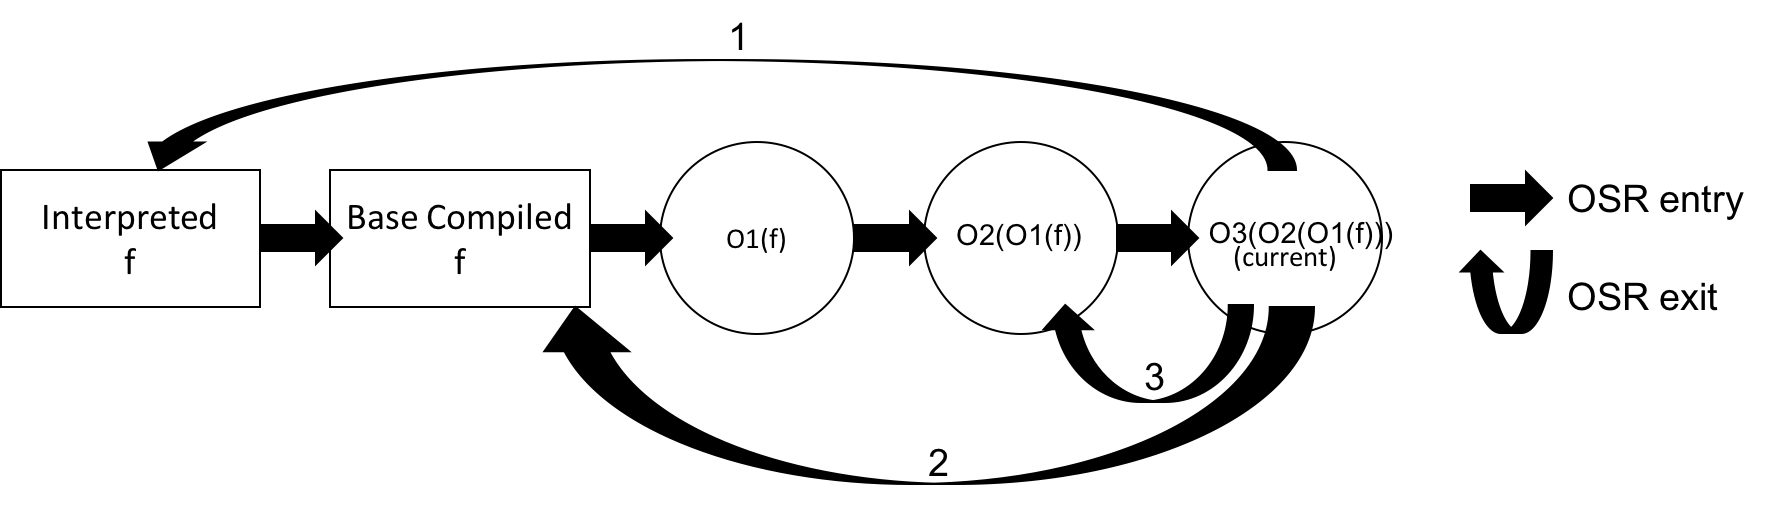
\includegraphics[scale=0.5]{Figures/wheretoexit}
\decoRule
\caption[OSR exit options]{OSR exit options.}
\label{OSR exit options}
\end{figure}

\subsubsection{The interpreter}
%List some examples that go to interpreter
%Good if have full control over the interpreter
%Bad for performance
A first option is to exit back to the interpreter. 
This approach has been taken by some virtual machines, such as Graal~\cite{duboscq2014speculation} or the Java HotSpot VM\cite{paleczny2001java} (see Section \ref{HotSpot} for more details).
This corresponds to the OSR exit 1 in Figure \ref{OSR exit options}.\\

Going back to the interpreter enables to have complete control over the execution environment.
The runtime framework has a fine-grained control over the interpreter state in which the execution is resumed.
This approach further gets rid of any assumption taken by the compiler and goes back to a safe environment.
Another way to put it would be to say that, since an assumption failed, the framework takes the conservative decision to go back to an assumption free environment to resume the execution.\\

Going back to the interpreter is a conservative approach that might impede the performance of the program.
The interpreted version of the function is assumed to be slow.
As a result, the function's execution will drastically slow down after exiting to the interpreter.
The question is then the following: can we provide the same correctness guarantees while exiting to a more efficient version of the function?\\

\subsubsection{The compiled base version}
%List some examples
%Better since its compiled. 
%Safe version of the code
%Still pretty slow.
Another option is to OSR exit to a base, compiled version of the function.
It corresponds to the OSR exit 2 in Figure \ref{OSR exit options}.
This is the approach taken by the WebKit framework~\cite{WebKitURL}(see section \ref{webkit}).
It represents a good intermediary between performance and complexity.
If the OSR framework does not have control over the execution environment, it requires careful instrumentation of the compiled code in order to properly propagate the execution state.
If the continuation function is generated on the fly, taking this OSR transition implies suffering the cost of compiling a proper continuation function.
On the other hand, the compiled version of the continuation function is expected to run faster than its interpreted equivalent.\\

On a theoretical point of view, going back to the base version avoids cascading OSR exits.
Since an exit was taken, it implies that one of the compiler's assumptions failed.
As it is hard to keep track of interferences and relations between different optimization steps, a profiler might not have the means to detect how one assumption's failure impacts other assumptions that were taken.
It might be the case that undoing one optimization yields an incorrect version of the code due to interferences between optimizations (in the worst case), or triggers other OSR exits.
An OSR exit also gives some feedback to the compiler's profiler that might improve the decisions taken for later speculative optimizations.
Restarting the optimization process from scratch might therefore yield a more performant version of the code, compared to the version obtained by undoing the optimization that failed.\\

\subsubsection{A less optimized version}
%List examples
%Try to keep good performances.
%Hard to generate the correct continuation function? Takes time might need to be done on the fly
A third option is to exit to an optimized version of the function that does not rely on the assumption that failed.
It corresponds to the OSR exit 3 in Figure \ref{OSR exit options}.
The function to which we exit is a fully optimized one, supposed to yield better performances than both the interpreted and the base versions.
This behavior can be observed in McOSR~\cite{lameed2013modular} (see section \ref{McOSR}) and OSR Kit~\cite{OSRKit}(see section \ref{describeOSRKit}).
This option strives to get the best possible performance, even in the presence of an assumption's failure.\\

As explained previously, there are two options to get the continuation function: either generate on the fly a new fully optimized version that does not rely on the assumption that failed, or "undo" the optimization that failed.
Undoing an optimization is hard, especially when it is intertwined with other transformations performed on the code.
An alternative is to keep the version of the code that was used to produce the optimized one, and use it as the continuation function for the OSR exit.
If the optimization that failed was the last transformation performed on the code, we exit to a version that already underwent all the available transformations and cannot be further optimized.
If that is not the case, we exit to a version of the code that is missing several optimizations.
For example, consider Figure \ref{OSR exit options}. 
If the assumption used for transformation $O3$ fails, we can easily exit to the version on which we applied the transformation, i.e., $O2(O1(f))$.
This corresponds to the OSR exit 3 in Figure \ref{OSR exit options}.
However, if the assumptions used for $O2$ fails, there is no previous version of $f$ that corresponds to $O3(O1(f))$ and generating one from $O3(O2(O1(f)))$ requires to undo $O2$.
Another solution, in that case, is to generate the continuation function on the fly.
Starting from $f$, we apply $O1$ and then $O3$, yielding $O3(O1(f))$.
This is a viable solution if and only if it is possible to find a mapping between $O3(O2(O1(f)))$ and $O3(O1(f))$.
If such a mapping does not exist, the compiler must ensure that no transformation messes with the OSR instrumentation.
In that case, we can always go back to the version on which we applied the transformation that failed, e.g., $O1(f)$ in our example.
OSR Kit, presented in section \ref{describeOSRKit}, can be used to implement such a solution.\\

\section{Constraints on the OSR Mechanism}
\subsection{The OSR Trade-Offs}\label{tradeOffs}
%Summary of all the trade offs exposed before

%OSR is a powerful technique, but requires to be tuned to our needs.
%as seen in this chapter, many design and implementation choices, might lead to very different results.
%Should cache or generate on the fly? How much reusability? How much performance gain?
%It has hard, if not impossible, to come up with one global solution.
On-stack replacement is a powerful technique that requires to be tailored to its use cases in order to exhibit good results.
As seen in this chapter, OSR can be implemented in several different ways, which in turn might lead to very sparse performance results.
For example, should the framework cache the compiled versions or should it generate the continuation functions on the fly?
This dilemma cannot be answered in the general case.
It depends on many conditions, among which the code reusability, i.e., what is the likelihood that the same continuation will be needed later during the program's execution?
There is also the trade-off between time and space complexities: caching increases the space usage, generating on the fly increases the time spent in the compiler.\\

The variety of performances that can be observed does not only depend on the design choices, or the target language, but also on the program's specificities.
A program with a certain profile might benefit from a specific OSR implementation, while another might be more amenable to another OSR design.
It is hard to know, before hand, which OSR implementation would yield the best results on a specific program, without having enough profiling information about the program's behavior. 
Furthermore, the program's behavior might depend on some runtime condition, and one OSR implementation is not guaranteed to be the most efficient in every run.  

\subsection{Limits on Optimizations}

The OSR instrumentation of the code limits the optimizations that the compiler can perform.
OSR points must be preserved by the compiler, for correctness, during the transformations.
Such instrumentation might increase variable live ranges, restrict code motion, or 
For example, in the Java HotSpot~\cite{paleczny2001java}, the instrumentation might extend the live range of variables, therefore preventing the compiler from removing them.
Another example is the SELF Debugger~\cite{holzle1992debugging}, which deoptimization process does not support tail call elimination and therefore does not implement it in the compiler.
Tail call elimination is a compiler optimization that enables, in the case of a tail call, to avoid allocating a new stack frame for the callee. 
It is commonly used to optimize tail call recursions.
The SELF debugger has no way of knowing how many stack frames were eliminated and is therefore unable to reconstruct them properly.
However, this limitation does not extend to every deoptimization implementation.
A carefully instrumented execution framework could keep track of state information and execution flow in order to enable tail call elimination OSR support.\\

OSR, and more specifically OSR exits, restricts code motion. 
In the case of deoptimization, the guarded OSR point protects some portion of code that must not be executed if the OSR exit is to be taken.
This implies that the compiler must not move any instruction that depends on this OSR exit condition above the OSR point.
The OSR instrumentation therefore limits code motion, which in turn might decrease the number of opportunities for compiler optimizations.